Let \(\mathcal{S}\) be the category of either simplicial sets or sufficiently nice topological spaces, e.g.~compactly generated weak Hausdorff spaces. When we talk about points or write \(x \in X\) the intended meaning is that \(x\) is a morphism \(1 \to X\). We denote the \(n\)-sphere in \(\mathcal{S}\) by \(\S^n\) and the one point space by \(1\). The internal hom of \(\mathcal{S}\) is written as \(\mathcal{S}(X, Y)\), reserving \(\Hom_{\mathcal{S}}(X, Y)\) for the external hom. We write \([X, Y] = \Hom_{\Ho(\mathcal{S})}(X, Y)\) for homotopy classes of maps (between bifibrant replacements). If \(X, Y\) are pointed, i.e.~are objects of \(\mathcal{S}_* = 1/\mathcal{S}\), we write \([X, Y]_*\) for the pointed-homotopy classes of basepoint-preserving maps; more properly \(\mathcal{S}_*\) acquires a model structure from \(\mathcal{S}\) in which the weak equivalences/fibrations/cofibrations are those whose underlying morphisms in \(\mathcal{S}\) is such, and \([X, Y]_* = \Hom_{\Ho(\mathcal{S}_*)}(X, Y)\).

\section{Homotopy (co)fibers}

For a set-function \(f : X \to Y\) and an element \(y \in Y\), one way of defining the fiber \(f^{-1}(y)\) is as the pullback of the cospan \(X \overset{f}{\to} Y \overset{y}{\leftarrow} 1\). In a model category we can define the ``homotopy fiber'' over \(y \in Y\) almost identically, except we take the homotopy pullback instead of the ordinary pullback. If we work with based spaces then we can unambiguously talk about \emph{the} homotopy fiber of a map, meaning the homotopy fiber with respect to the basepoint. The dual notion of a homotopy cofiber requires no choice of point \(y \in Y\), it is simply the homotopy pushout of the span \(Y \overset{f}{\leftarrow} X \to 1\) where the right map is uniquely determined.

\section{Truncation and connectedness}

We say an object \(X\) of \(\mathcal{S}\) is \(n\)-truncated if \(\pi_k(X, x) = 0\) for all basepoints \(x \in X\) and \(k > n\). Truncated-ness has a relative variant: a morphism \(f : X \to Y\) is \(n\)-truncated when its homotopy fiber over any point \(y \in Y\) is \(n\)-truncated. The homotopy fiber of \(X \to 1\) is a fibrant replacement of \(X\), so we find \(X\) is \(n\)-truncated iff \(X \to 1\) is \(n\)-truncated.

\paragraph{Examples}

\begin{itemize}
\tightlist
\item
  Because the universal cover of \(\S^1\) is contractible we know (by the long exact sequence in homotopy groups of a fibration) that \(\pi_k(\S^1) = 0\) for \(k > 1\), i.e.~\(\S^1\) is \(1\)-truncated.
\item
  The sphere \(\S^n\) can never be \(k\)-truncated for \(k < n\), since \(\pi_n(\S^n) \neq 0\). The existence of the hopf fibration tells us \(\S^2\) is not \(2\)-truncated.
\item
  The hopf fibration \(\S^3 \to \S^2\) is itself \(1\)-truncated, since it is a circle bundle (the homotopy fiber of a fibration is its ordinary fiber).
\item
  By examining the cohomology of Eilenberg-MacLane spaces Serre was able to establish that a simply connected finite space \(X\) (in the sense defined below) with nonzero reduced cohomology mod \(p\) (for some prime \(p\)) has infinitely many nonzero homotopy groups, i.e.~is not \(k\)-truncated for any \(k\). (In particular this is true for the spheres above dimension \(1\)).
\item
  The nerve of a groupoid is always \(1\)-truncated.
\item
  An Eilenberg-MacLane space \(K(G, n)\) is (definitionally) \(n\)-truncated.
\end{itemize}

The dual notion to a space being \(n\)-truncated is that it is \(n\)-connected. For \(n \geq 0\) we say \(X\) is \(n\)-connected if \(X\) is nonempty and \(\pi_k(X, x) = 0\) for all \(k \leq n\) for all \(x \in X\). By convention we define \((-1)\)-connected to mean that \(X\) is inhabited (nonempty), and we call every space \((-2)\)-connected. In low dimensions this recovers familiar notions: \(0\)-connected means path connected and \(1\)-connected means simply connected. The \(n\)-sphere is \((n - 1)\)-connected. Connectivity also has a relative version: a continuous map \(f : X \to Y\) is \(n\)-connected if its homotopy fiber at every \(y \in Y\) is \((n - 1)\)-connected (all maps are \((-1)\)-connected). The reason for the degree shift is that relative connectedness is related to connectedness of spaces in the dual way to how relative truncatedness is related to truncatedness of spaces; while it is the case that a space \(X\) is \(n\)-connected iff the map \(X \to 1\) is \((n+1)\)-connected, the more worthwhile condition is that for a basepoint \(x \in X\) the inclusion \(x : 1 \to X\) is \(n\)-connected iff \(X\) is \(n\)-connected. To see this we note that the homotopy fiber of \(x : 1 \to X\) at a point \(y \in X\) is the space of paths from \(x\) to \(y\) in \(X\) (essentially by definition of the homotopy fiber/homotopy pullback); if \(X\) is not \(0\)-connected then there is some \(y\) for which this fiber is empty, hence not \((-1)\)-connected, and if \(X\) is \(0\)-connected then the homotopy fiber at any point may be identified with \(\Omega(X, x)\), and since \(\pi_i(\Omega X) \cong \pi_{i+1}(X)\) we find \(X\) is \(n\)-connected iff the homotopy fibers are \((n-1)\)-connected.

A more concrete definition of \(n\)-connectedness of a map is that \(f : X \to Y\) is \(n\)-connected (\(n \geq 0\)) iff for every \(x \in X\) and \(i < n\) the induced map \(f_* : \pi_i(X, x) \to \pi_i(Y, f(x))\) is an isomorphism, while \(f_* : \pi_n(X, x) \to \pi_n(Y, f(x))\) is an epimorphism. The \(n = 0\) case says \(f\) is a surjection on path components, which is easily seen to be equivalent to the homotopy fibers of \(f\) all being \((-1)\)-connected (nonempty). For higher levels we use the homotopy fiber sequence \(F \to X \to Y\) and the long exact sequence of a fibration/fiber sequence.

\section{Smashing}

The category of pointed sets/simplicial sets/topological spaces has an internal hom derived from the internal hom of the original category. Specifically the new internal hom will be the pullback
\[
\begin{tikzcd}
\mathcal{S}_*((X, x_0), (Y, y_0)) \arrow[r, hook] \arrow[d] \arrow[dr, phantom, "\lrcorner" very near start] & \mathcal{S}(X, Y) \arrow[d, "f \mapsto f(x_0)"] \\
1 \arrow[r, "y_0"'] & Y
\end{tikzcd}
\]
or in other words it's the (strict) fiber of the evaluation at \(x_0\) map \(\mathcal{S}(X, Y) \to Y\) over \(y_0 \in Y\). The basepoint \(1 \to \mathcal{S}_*((X, x_0), (Y, y_0))\) is the map induced by the identity \(1 \to 1\) and the map \(1 \to \mathcal{S}(X, Y)\) picking out the constant function \(\overline{y_0}\) at \(y_0\). It turns out that this internal hom has a left adjoint, hence \(\mathcal{S}_*\) is a (symmetric) monoidal closed category. We work backwards to determine the tensor. For pointed sets \((X, x_0), (Y, y_0)\) we want an object that corepresents the functor \((Z, z_0) \mapsto \Hom_{\cat{Set}_*}((X, x_0), \mathcal{S}_*((Y, y_0), (Z, z_0)))\). Giving a map \((X, x_0) \to \mathcal{S}_*((Y, y_0), (Z, z_0))\) is the same as giving a map \(X \to \mathcal{S}(Y, Z)\) valued in the fiber over \(z_0\) and which sends \(x_0\) to the constant map at \(z_0\) (all interpreted diagrammatically). But this is the same as giving a map \(\varphi : X \times Y \to Z\) making the diagram
\[
\begin{tikzcd}
X \arrow[r, "{(\id, y_0)}"] \arrow[dr, "\overline{z_0}"'] & X \times Y \arrow[d, "\varphi"] & Y \arrow[l, hook', "{(x_0, \id)}"'] \arrow[dl, "\overline{z_0}"] \\
& Z &
\end{tikzcd}
\]
commute. In other words, a morphism \((X, x_0) \to \mathcal{S}_*((Y, y_0), (Z, z_0))\) is the same thing as a morphism \(X \times Y \to Z\) which sends the entire wedge sum \(X \vee Y = (X \times \{y_0\}) \cup (\{x_0\} \times Y)\) to \(z_0\). The equation defining \(X \vee Y\) doesn't properly make sense if \(X, Y\) are simplicial sets, but we can interpret it as the image of a map \(X \coprod Y \to X \times Y\). The \emph{smash product} of \((X, x_0)\) and \((Y, y_0)\) is defined to be \(X \wedge Y = (X \times Y)/(X \vee Y)\), with basepoint the class of \(X \vee Y\), and since all those ``same thing as''es above are really natural isomorphisms this shows \(X \wedge Y\) represents the desired functor, and \(- \wedge -\) is left adjoint to \(\mathcal{S}_*(-, -)\). Again some care must be taken in interpreting the equation \(X \wedge Y = (X \times Y)/(X \vee Y)\), what we mean is the pushout of the inclusion \(X \vee Y \to X \times Y\) with the terminal map \(X \vee Y \to 1\), and the structure map \(1 \to X \wedge Y\) is the basepoint. The important thing about \(X \wedge Y\) in our argument was the universal map \(X \times Y \to X \wedge Y\) and that its dual \(\Hom_{\mathcal{S}}(X \wedge Y, -) \to \Hom_{\mathcal{S}}(X \times Y, -)\) identified the domain with the morphisms out of \(X \times Y\) killing \(X \vee Y\), which is all formal from the definition as a pushout. The unit of the smash product is the two-point space or zero-sphere \(\S^0\); this is equivalent under the adjunction to the assertion that \(X \to \mathcal{S}_*(\S^0, X)\) is an isomorphism, which holds because the map \(\mathcal{S}_*(\S^0, X) \to X\) given by evaluation at the non-basepoint of \(\S^0\) is its inverse. We don't prove it here, but the smash product respects weak equivalences (for topological spaces this needs the basepoints to be nondegenerate, i.e.~the spaces to be well-pointed; for simplicial sets it always holds) and so descends to a symmetric monoidal structure on the homotopy category of pointed spaces. It is true (but perhaps not obvious) that the smash product naturally distributes over the wedge sum.

A fun note is that if \(A, B\) are abelian groups and we consider them as sets based at \(0\), the canonical map \(A \times B \to A \otimes B\) factors through \(A \wedge B\); this just says \(a \otimes 0 = 0 \otimes b = 0\).

\section{Suspension and loop spaces}

For an object \(X\) of a model category we define the \emph{suspension} of \(X\) to be the homotopy pushout of \(1 \leftarrow X \rightarrow 1\). If \(X\) has a basepoint \(x_0 : 1 \to X\) we define the loop space at \(x_0\) to be the homotopy pullback of \(1 \rightarrow X \leftarrow 1\). In other words, the loop space is the homotopy fiber of \(1 \to X\). In general these are only defined up to weak equivalence in the original model category, but they define adjoint functors on the homotopy category of pointed objects. Since the adjunction only exists at the level of pointed objects, it's typical to restrict attention to the case of a pointed model category (one where the initial and terminal object coincide and hence each object has a unique pointing). In the case of unbased topological spaces it's common to call the homotopy pushout \(1 \leftarrow X \rightarrow 1\) the ``unreduced suspension''.

In the particular case of pointed simplicial sets (or topological spaces) we can define functorial choices of suspension/loop space in terms of the internal hom and smash product defined previously. The suspension is \(\Sigma X = \S^1 \wedge X\) and the loop space is the internal hom \(\Omega X = \mathcal{S}_*(\S^1, X)\) (the way we make \(\mathbb{S}^1\) into a based space doesn't matter too much, but for concreteness we take \(\S^1 = \Delta^1/\partial\Delta^1\) to be the minimal model of the simplicial circle, which has a unique vertex, and \(\S^n = (\S^1)^{\wedge n}\)). The adjunction \(\Sigma \dashv \Omega\) then exists before passing to the homotopy category, and one can check it is a Quillen adjunction (this follows easily from our unproven assertion that smashing respects weak equivalence, as \(\Sigma\) easily preserves cofibrations/monomorphisms and this tells us it preserves acyclic cofibrations as well).

Since \(\Omega\) is a right Quillen functor, \(\mathcal{S}_*(\S^1, X)\) is only guaranteed to be the appropriate homotopy pullback when \(X\) is fibrant. Every topological space is fibrant, but a simplicial set is fibrant only when it is a Kan complex, and for a general \(X\) we must first replace \(X\) fibrantly. For example \(\S^1 = \Delta^1/\partial\Delta^1\) is not a Kan complex, and \(\mathcal{S}_*(\S^1, \S^1)\) has only two vertices, while \(\pi_0(\Omega \S^1) \cong \Z\). For fibrant \(X\), the fact that \(\mathcal{S}_*(\S^1, X)\) is the appropriate homotopy pullback follows from the fact that the path space projection \(PX \to X\) is a fibrant replacement of the inclusion \(1 \to X\), as \(\mathcal{S}_*(\S^1, X)\) is the strict fiber of this fibration (hence the homotopy fiber of the original map); here \(PX\) is the space of paths in \(X\) starting at \(x_0\), i.e.~the fiber of the evaluation map \(\mathcal{S}(\Delta^1, X) \to X\) over \(x_0\). The fact that \(\Sigma X\) gives the correct homotopy pushout then follows from the derived adjunction on the level of the homotopy category and the uniqueness of adjoints.

Suspension behaves extremely well with spheres, in that \(\Sigma \S^n \cong \S^{n+1}\) (we already know the \(n = 0\) case, by the fact that \(\S^0\) is a unit for the smash product). We give some pictures in the topological space model that hopefully provide intuition for this, and for the suspension more generally.
\begin{center}
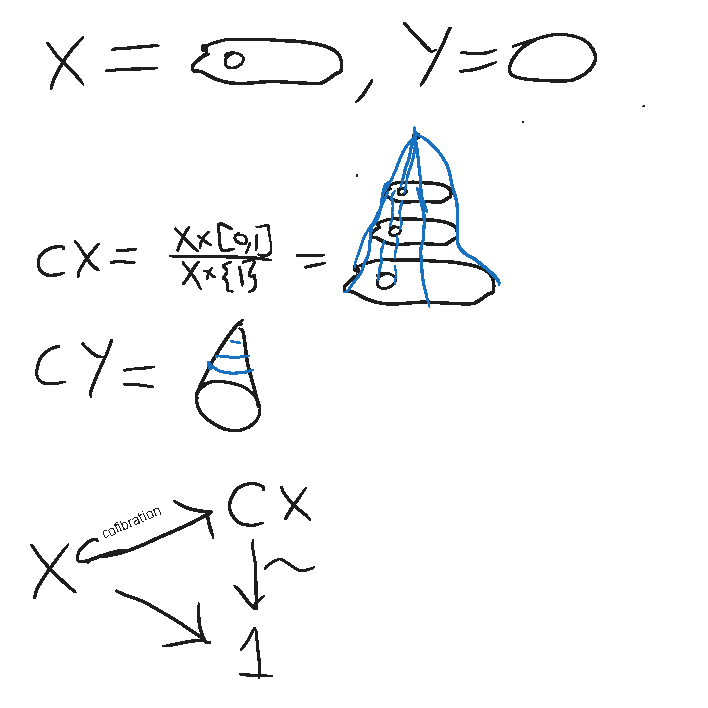
\includegraphics[scale=0.8]{figures/cones}
\end{center}
\begin{center}
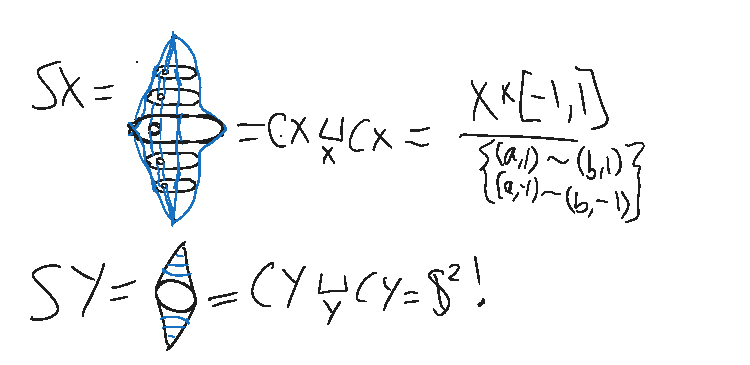
\includegraphics[scale=0.8]{figures/suspension}
\end{center}
\begin{center}
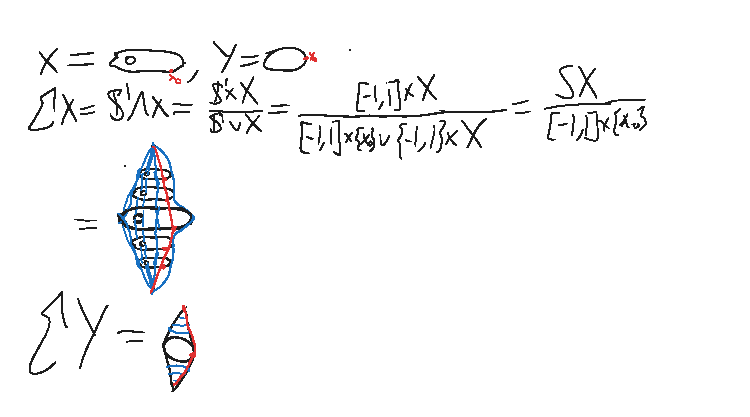
\includegraphics[scale=0.8]{figures/reduced_suspension}
\end{center}
Using the equation \(\Sigma \S^n \cong \S^{n+1}\) (and its ``filled in version'' that the suspension of the \(n\)-disk is the \((n+1)\)-disk) and the fact that every CW complex is built from spheres, we find that suspending a CW complex has the effect of raising the dimension of each cell other than the basepoint by one. All we're doing from this perspective is reindexing!

Now observe that \[\pi_n(X, x_0) = [\S^n, X]_* = [\Sigma^n \S^0, X]_* = [\S^0, \Omega^n X]_* = \pi_0(\Omega^n X).\]
In this way the group structure of \(\pi_n\) can be seen as arising from a group structure on \(\Omega^n X\) in \(\Ho(\mathcal{S})\) and the fact that \(\pi_0\) preserves finite products. We focus on the \(n = 1\) case for now, which is sufficient for the group structure on all \(n\). The multiplication operation on the fundamental group is originally defined as explicit concatenation operation on paths, and this concatenation is a continuous function \(\Omega X \times \Omega X \to \Omega X\). Of course this operation isn't associative, but the homotopy class of it defines an associative multiplication on \(\Omega X\) in \(\Ho(\mathcal{S})\), and the homotopy class of the basepoint \(1 \to \Omega X\) (the constant map at \(x_0\)) is an identity for this multiplication. Thus \(\Omega X\) has the structure of a group object in \(\Ho(\mathcal{S})\). Concatenation is a based map and all of these homotopies fix the constant loop, so \(\Omega X\) is in fact a group object in \(\Ho(\mathcal{S}_*)\). With a little more work we can replace \(\Omega X\) with a homotopy equivalent space which is a \emph{strict} monoid (the inversion map is still only an inverse up to homotopy). The idea there is to allow our paths to take arbitrary real length instead of normalizing to length \(1\).

The equation \(\pi_n(X, x_0) = \pi_0(\Omega^n X)\) also tells us that \(\pi_n(\Omega X) = \pi_{n+1}(X)\), so \(\Omega\) has the effect of shifting the homotopy groups of \(X\) down by \(1\). Suspension doesn't have quite as nice a relation with homotopy groups, but the Mayer-Vietoris theorem (or axiom) tells us that \(\Sigma\) has the effect of shifting the (co)homology groups up by \(1\) (for any reduced (co)homology theory). Additionally the action of \(\Sigma\) on morphisms gives a group homomorphism, called the suspension homomorphism, \[\pi_n(X) = [\S^n, X]_* \to [\Sigma \S^n, \Sigma X]_* = [\S^{n+1}, \Sigma X]_* = \pi_{n+1}(\Sigma X).\]Suspension also \emph{raises connectivity}, meaning if \(X\) is \(n\)-connected then \(\Sigma X\) is \((n+1)\)-connected. It's easy to see that \(\Sigma X\) is always \(0\)-connected, and if \(X\) is \(0\)-connected then we can show \(\Sigma X\) is \(1\)-connected by the Seifert-Van Kampen theorem (this is easiest imo by working with the homotopy equivalent unreduced suspension and the decomposition of that space into two cones). If we know \(X\) is \(1\)-connected to start with then we have a much cheaper argument that \(\Sigma X\) has \(1\) level more of connectivity, namely we use the Hurewicz theorem and the fact that suspension shifts homology up by \(1\). It's also true that suspending a morphism raises its connectivity by \(1\). When the spaces involved are connected this is the same argument applied to relative homology: \(\Sigma X\) and \(\Sigma Y\) are simply connected, suspension shifts the relative homology of \(f : X \to Y\) up by \(1\), and the relative Hurewicz theorem turns this back into a statement about homotopy groups (the disconnected case needs Seifert-Van Kampen again in low degrees).

\section{Freudenthal suspension theorem}

Theorem: If \(X\) is \(n\)-connected then the unit \(X \to \Omega \Sigma X\) is \((2n+1)\)-connected.

Note: We can identify \(\pi_i(\Omega \Sigma X) = \pi_{i + 1}(\Sigma X)\) and under this identification the map \(\pi_i(X) \to \pi_{i+1}(\Sigma X)\) induced by the unit is the suspension homomorphism. Also, this theorem has a beautiful ``synthetic'' proof in Homotopy Type Theory.

Proof sketch: Argue the \(n = 0\) case ``by hand'' (up to some identification the suspension homomorphism is the Hurewicz map \(\pi_1(X) \to H_1(X)\)). For \(n > 0\), \(X\) and \(\Omega \Sigma X\) are both simply connected. Strictify \(\Omega \Sigma X\) to a topological monoid \(\Omega_m \Sigma X\) as discussed before. The unit \(X \to \Omega_m \Sigma X\) gives rise to a monoid homomorphism from the free monoid \(J(X)\) on \(X\) to \(\Omega_m \Sigma X\) (we want the free monoid on \(X\) as a \emph{pointed} set here, so the identity is the point of \(X\) and not the empty word). We define the free monoid as a quotient of a disjoint union of powers of \(X\), so it acquires a topology. Argue that the monoid homomorphism \(J(X) \to \Omega_m \Sigma X \simeq \Omega \Sigma X\) is a homology isomorphism (with coefficients in every field, hence also integrally) by explicitly calculating the homology of \(J(X)\) (this is not so hard if we filter \(J(X)\) by the length of words and use the Kunneth formula, we get that it's the tensor algebra on the reduced homology of \(X\)) and \(\Omega\Sigma X\) (we use the relationship between the loop space and the path space, which is contractible, either using the Serre spectral sequence or more geometrically decomposing \(\Sigma X\) into two cones, pulling these back to the path space, and applying the Mayer-Vietoris theorem in clever ways; we get recursive nonlinear relations between the higher and lower degree homology and use the algebra structure induced from the monoid structure of \(\Omega_m \Sigma X\) to deduce from the recurrence relations that the homology is the tensor algebra). By the (relative) Hurewicz theorem we find that the map \(J(X) \to \Omega \Sigma X\) is a weak equivalence factoring the unit through the inclusion \(X \subseteq J(X)\). Then using the length-filtration on \(J(X)\) we write \(X \to J(X)\) as a transfinite composite \[X = J(X)_{\leq 1} \to J(X)_{\leq 2} \to J(X)_{\leq 3} \to \cdots \to J(X).\]It then suffices to show each inclusion \(J_{\leq i}(X) \to J_{\leq i+1}(X)\) is \((2n+1)\)-connected, and these inclusions are much easier to understand.

There are several reformulations of the Freudenthal suspension theorem, which are all essentially equivalent. Freudenthal's original formulation that the suspension morphism \(\pi_{n+k}(\S^n) \to \pi_{n+k+1}(\S^{n+1})\) is an isomorphism if \(n > k + 1\). When discussing the homotopy groups of spheres \(\pi_i(\S^n)\) the range of indices \(i, n\) such that \(2n > i + 1\) is called the ``stable range'', because this theorem tells us that as we raise both indices the group will ``stabilize'' once \(2n > i + 1\). This version holds by interpreting the unit (or its induced map on homotopy groups) as the suspension homomorphism, and more generally that map \(\pi_k(X) \to \pi_{k + 1}(\Sigma X)\) is an isomorphism for \(k \leq 2n\), if \(X\) is an \(n\)-connected space. We can also generalize the space we map out of: if \(X\) is a pointed \(n\)-connected space and \(Y\) is a pointed space of dimension \(\leq 2n\) (so as a simplicial set all nondegenerate simplices of \(Y\) have dimension \(\leq 2n\), or as a CW complex all cells have dimension \(\leq 2n\)) then the action of the suspension functor \([Y, X]_* \to [\Sigma Y, \Sigma X]_*\) is a bijection.

This follows from the formulation about homotopy groups and the fact that \(Y\) is built from cells of dimension \(\leq 2n\), so the \((2n+1)\)-connected unit \(X \to \Omega \Sigma X\) induces a bijection \([Y, X]_* \to [Y, \Omega \Sigma X]_* \cong [\Sigma Y, \Sigma X]_*\). Since suspension raises both the connectivity and the dimension of a space by \(1\), if we start with any connected space \(X\) and \emph{finite} space \(Y\) of dimension \(d\) then \(\Sigma^d Y\) is \(2d\)-dimensional while \(\Sigma^d X\) is \(d\)-connected, hence any further suspension doesn't change the mapping space \([\Sigma^d Y, \Sigma^d X]_*\). Thus if \(X, Y\) are both finite spaces (meaning they have finitely many nondegenerate simplices in the simplicial set model or that they have finitely many cells in the CW complex version) the sequence \[[X, Y]_* \to [\Sigma X, \Sigma Y]_* \to [\Sigma^2 X, \Sigma^2 Y]_* \to [\Sigma^3 X, \Sigma^3 Y]_* \to\ \cdots\]stabilizes (in the sense that after some finite stage the maps become isomorphisms).

\section{The Spanier-Whitehead category}

Let \(\mathcal{S}_{f}\) be the category of finite spaces, or spaces weak homotopy equivalent to finite spaces. We discussed before what this means concretely, and we can define it internal to \(\mathcal{S}\) by saying it's the closure of \(\{1\}\) under finite homotopy colimits\footnote{This is \emph{almost} the same as the compact objects, and in fact there would be no issue defining the Spanier-Whitehead category if we took all compact objects, but it's possible to have a retract of a finite space which is not itself finite. This is possible despite the closedness under finite homotopy colimits because, unlike for \(1\)-categories, splitting idempotents in an \((\infty, 1)\)-category requires taking an infinite colimit. There is a class called ``Wall's finiteness obstruction'' valued in an algebraic \(K\)-theory group which vanishes for a compact object if and only if it is a genuine finite homotopy type.} (or simply by homotopy pushouts and the initial object). We define the pre-Spanier-Whitehead category \(\mathcal{SW}_+\) to have as objects the pointed objects of \(\mathcal{S}_f\), which we write \(\mathcal{S}_{f,*}\), and have hom-sets \[\Hom_{\mathcal{SW}_+}(X, Y) = \colim\limits_{r \geq 0}\ [\Sigma^r X, \Sigma^r Y]_*.\]In fact, if we use the same colimit but with internal homs of pointed spaces, i.e.~\[\mathcal{SW}_+(X, Y) = \colim\limits_{r \geq 0}\ \mathcal{S}_*(\Sigma^r X, \Sigma^r Y)\]we can make \(\mathcal{SW}_+\) an \(\mathcal{S}_*\)-enriched or (by forgetting structure) \(\mathcal{S}\)-enriched category; this has homotopy category the ordinary category we're denoting \(\mathcal{SW}_+\), which means that \(\pi_0(\mathcal{SW}_+(X, Y)) \cong \Hom_{\mathcal{SW}_+}(X, Y)\). The identity is the class of the identity map (in any degree) and composition is defined by taking representatives \(f : \Sigma^r Y \to \Sigma^r Z\) and \(g : \Sigma^s X \to \Sigma^s Y\) and producing the class of \(\Sigma^s f \circ \Sigma^r g\), or of \(\Sigma^{\max(r, s) - r} f \circ \Sigma^{\max(r, s) - s} g\). The Freudenthal suspension theorem says that for any \(X\) there is a constant \(c = \dim X + 2\) such that the canonical morphism \([\Sigma^c X, \Sigma^c Y] \to \Hom_{\mathcal{SW}_+}(X, Y)\) is a bijection for any \(Y\). In fact it's better than a bijection, it's an isomorphism of abelian groups; we can write the terms in the colimit as \[[\Sigma^r X, \Sigma^r Y]_* \cong [X, \Omega^r \Sigma^r Y]_* \cong \pi_r(\mathcal{S}_*(X, \Sigma^r Y))\]and for \(r \geq 2\) these terms have a natural abelian group structure and as mentioned prior the action of \(\Sigma\) is a group homomorphism. However in the enriched context the canonical morphisms \(\mathcal{S}_*(\Sigma^r X, \Sigma^r Y) \to \mathcal{SW}_+(X, Y)\) are \emph{not} eventually weak equivalences. The issue is one of uniformity. For fixed \(i\) the induced maps \(\pi_i(\mathcal{S}_*(\Sigma^r X, \Sigma^r Y)) \to \pi_i(\mathcal{SW}_+(X, Y))\) are \(r\)-eventually isomorphisms, but there's no sufficiently large \(r\) such that they are isomorphisms for every \(i\). Explicitly the issue is that if we fix \(r\) and vary \(i\) we see
\begin{align*}
\pi_i(\mathcal{S}_*(\Sigma^r X, \Sigma^r Y)) &= [\S^i, \mathcal{S}_*(\Sigma^r X, \Sigma^r Y)]_* \\
&= [\S^i \wedge \Sigma^r X, \Sigma^r Y]_* = [\Sigma^{i+r} X, \Sigma^r Y]_*
\end{align*}
and the Freudenthal suspension theorem will not apply as \(i \to \infty\) since the dimension of \(\Sigma^{i+r} X\) grows without bound while the connectivity of \(\Sigma^r Y\) remains constant. However the maps \(\mathcal{S}_*(\Sigma^r X, \Sigma^r Y) \to \mathcal{S}_*(\Sigma^{r+1} X, \Sigma^{r+1} Y)\) are raising in connectivity, since the suspension theorem tells us \(\pi_i(\mathcal{S}_*(\Sigma^r X, \Sigma^r Y)) \to \pi_i(\mathcal{S}_*(\Sigma^{r+1} X, \Sigma^{r+1} Y))\) is an isomorphism when \(\dim X + i + r \leq 2(r - 1)\), i.e.~when \(r \geq i + \dim X + 2\).

Since \(\Obj(\mathcal{S}_{f,*}) = \Obj(\mathcal{SW}_+)\) and there's a natural map \(\Hom_{\mathcal{S}_*}(X, Y) \to \Hom_{\mathcal{SW}_+}(X, Y)\) we have a functor \(\Sigma^\infty : \mathcal{S}_{f,*} \to \mathcal{SW}_+\) which is the identity on objects and this latter map on morphisms (one way to think of this action on morphisms is as the transfinite composition of the suspension homomorphism with itself). From now on we will ``forget'' that \(\mathcal{S}_{f,*}\) and \(\mathcal{SW}_+\) have the same objects, instead writing \(\Sigma^\infty X\) for the object of \(\mathcal{SW}_+\) corresponding to \(X\). The endofunctor \(\Sigma : \mathcal{S}_* \to \mathcal{S}_*\) extends to an endofunctor of \(\mathcal{SW}_+\), where \(\Sigma^\infty \circ \Sigma = \Sigma \circ \Sigma^\infty\), and it's easy to see \(\Sigma : \mathcal{SW}_+ \to \mathcal{SW}_+\) is fully faithful. One way we can interpret the suspension theorem is that for any objects \(X, Y\) of \(\mathcal{S}_{f,*}\) there is some finite \(r\) such that \(\Sigma^\infty : \Hom_{\Ho(\mathcal{S}_*)}(\Sigma^r X, \Sigma^r Y) \to \Hom_{\mathcal{SW}_+}(\Sigma^\infty X, \Sigma^\infty Y)\) is an isomorphism.

One of the most important objects in the Spanier-Whitehead category is the sphere spectrum \(\S = \Sigma^\infty \S^0\) and its suspensions \(\Sigma^r \S\). The group \(\Hom_{\mathcal{SW}_+}(\Sigma^r \S, \Sigma^\infty X)\) is called the \(r\)th \emph{stable homotopy group} of \(\Sigma^\infty X\), defined by \(\pi^{\mathrm{st}}_r(X) = \colim_{s \geq 0} \pi_{r+s}(\Sigma^s X)\). The most basic form of the Freudenthal suspension theorem is that the stable homotopy groups of spheres equal the unstable ones in the stable range! It turns out that these stable homotopy groups are much easier to study than the ordinary unstable homotopy groups, and in general stable phenomena (invariants defined on the Spanier-Whitehead category) are easier to understand than unstable ones. Two spaces become isomorphic in the Spanier-Whitehead category if they are \emph{stably homotopy equivalent}, and a continuous map \(f : X \to Y\) becomes an isomorphism if it induces an isomorphism on all stable homotopy groups.

The full Spanier-Whitehead category \(\mathcal{SW}\) is like \(\mathcal{SW}_+\), but we add in formal desuspensions of the objects. Explicitly the objects are pairs \((X, n)\) where \(X\) is a finite pointed space and \(n \in \Z\), interpreted formally as \(\Sigma^n X\), and hom-sets are given by \[\Hom_{\mathcal{SW}}((X, n), (Y, m)) = \colim\limits_{r \geq \max(0, -n, -m)}\ [\Sigma^{n + r} X, \Sigma^{m + r} Y]_*.\]Again we can interpret this with internal homs and get an \(\mathcal{S}_*\)-enrichment. We view \(\mathcal{SW}_+\) as the full subcategory of \(\mathcal{SW}\) on objects with \(n = 0\) and write \(\Sigma^\infty X = (X, 0)\). For \(n \geq 0\) the class of the identity map \(\Sigma^{0+0} \Sigma^n X \to \Sigma^{n+0} X\) defines an element of the group \(\Hom_{\mathcal{SW}}((\Sigma^n X, 0), (X, n))\), and the identity the other way a morphism going the other way, and these give an isomorphism \((\Sigma^n X, 0) \cong (X, n)\) between the actual suspension in degree \(0\) and the formal suspension. This allows us to set \(\Sigma (X, n) = (X, n+1)\) and know we extend the suspension of \(\mathcal{SW}_+\) and that \(\Sigma \circ \Sigma^\infty = \Sigma^\infty \circ \Sigma\), up to isomorphism. In addition this tells us the closure of \(\mathcal{SW}_+ \subseteq \mathcal{SW}\) under isomorphism contains all objects \((X, n)\) where \(n \geq 0\). So we can interpret \(\mathcal{SW}\) as the colimit (strictly or non-strictly, it doesn't matter since it's really just a union) of categories \[\mathcal{SW}_+ \overset{\Sigma}{\to} \mathcal{SW}_+ \overset{\Sigma}{\to} \mathcal{SW}_+ \overset{\Sigma}{\to} \cdots\]This is analogous to defining the category of bounded chain complexes (or more properly the compact objects of the derived category) as the colimit of the connective chain complexes (connective complexes of fg projectives) under left shifts by one. It's immediate from our definition of the suspension on \(\mathcal{SW}\) that it is an autoequivalence, with inverse \(\Omega (X, n) = (X, n - 1)\). We also again have (stable) homotopy groups defined by \(\pi_i(X) = \Hom_{\mathcal{SW}}(\Sigma^i \S, X)\), where now \(i \in \Z\) can be negative.

The wedge sum of pointed spaces respects weak equivalence and since the smash product distributes over it we have \(\Sigma (X \vee Y) = \Sigma X \vee \Sigma Y\), so intuitively it should lift to the Spanier-Whitehead category. It's not hard to extend it to \(\mathcal{SW}_+\) by setting \(\Sigma^\infty X \vee \Sigma^\infty Y = \Sigma^\infty (X \vee Y)\), and more generally on \(\mathcal{SW}\) by \[(X, n) \vee (Y, m) = \left(\Sigma^{n - \min(n, m)} X \vee \Sigma^{m - \min(n, m)} Y, \min(n, m)\right).\]The degree shifting may seem odd, but this equation is forced on us by the identities \(\Sigma (X \vee Y) = \Sigma X \vee \Sigma Y\) and \(\Sigma^\infty X \vee \Sigma^\infty Y = \Sigma^\infty (X \vee Y)\). The wedge sum is the coproduct in the category of pointed spaces, and it's not hard to deduce from this that it's the coproduct in \(\mathcal{SW}_+\) as well. Since \(\mathcal{SW}_+\) generates \(\mathcal{SW}\) under (de)suspension and \(\vee\) commutes with suspension, we can deduce from this that \(\vee\) is the coproduct in \(\mathcal{SW}\). Because \(\mathcal{SW}\) is \(\cat{Ab}\)-enriched a formal argument implies \(\vee\) is also the categorical product.

Similarly we can define \((X, n) \wedge (Y, m) = (X \wedge Y, n + m)\), and it will satisfy \[\Sigma^\infty (X \wedge Y) = \Sigma^\infty X \wedge \Sigma^\infty Y\]and \(\S \wedge X = X\) and \(\Sigma X \wedge Y = X \wedge \Sigma Y = \Sigma (X \wedge Y)\). This is functorial because the smash product respects weak equivalence, hence descends \(\Ho(\mathcal{S}_*)\), and \[\Sigma^n X \wedge \Sigma^m Y = (\S^n \wedge X) \wedge (\S^m \wedge Y) = (\S^n \wedge \S^m) \wedge (X \wedge Y) = \Sigma^{n+m}(X \wedge Y).\]Thus given elements of \(\Hom_{\mathcal{SW}}((X, n), (X', n'))\) and \(\Hom_{\mathcal{SW}}((Y, m), (Y', m'))\), represented by \(f : \Sigma^{n+r} X \to \Sigma^{n'+r} X'\) and \(g : \Sigma^{m+s} Y \to \Sigma^{m'+s} Y'\), we have a smash product \(f \wedge g : \Sigma^{(n+m)+(r+s)} (X \wedge Y) \to \Sigma^{(n'+m')+(r+s)} (X' \wedge Y')\) which defines an element of \(\Hom_{\mathcal{SW}}((X \wedge Y, n + m), (X' \wedge Y', n' + m'))\). This needs a sign to be well defined: replacing \(g\) by \(\Sigma g\), which represents the same morphism, moves the new suspension coordinate past \(\S^{n+r}\) in the source and past \(\S^{n'+r}\) in the target, and since the twist map of \(\S^a \wedge \S^1\) has degree \((-1)^a\) this changes the class of \(f \wedge g\) by \((-1)^{n+n'}\). So we define the smash product of the two morphisms to be \((-1)^{(n+n')s}\) times the class of \(f \wedge g\). Similarly the symmetry isomorphism \((X, n) \wedge (Y, m) \cong (Y, m) \wedge (X, n)\) must include the sign \((-1)^{nm}\) coming from the twist map of \(\S^n \wedge \S^m\). With these signs the symmetric monoidal structure on \(\wedge\) at the level of \(\mathcal{S}_*\) descends to give \(\mathcal{SW}\) the structure of a symmetric monoidal category; Adams' \emph{Stable Homotopy and Generalised Homology}, Part III, treats this carefully.

\section{Fiber and cofiber sequences}

We discussed previously the notion of the homotopy cofiber of a map of topological spaces. We can extend this notion to the category \(\mathcal{SW}\): because \(\Sigma\) on \(\mathcal{S}_*\) is a left quillen functor it preserves the homotopy cofiber, i.e.~if \(f : X \to Y\) is a based map and \(g : Y \to Z\) is a homotopy cofiber of \(f\) then \(\Sigma g : \Sigma Y \to \Sigma Z\) is a homotopy cofiber of \(\Sigma f : \Sigma X \to \Sigma Y\). Furthermore in this setup there is an essentially unique map \(Z \to \Sigma X\) induced by the (homotopy) universal property of the (homotopy) cofiber; both \(Z\) and \(\Sigma X\) are pushouts and there is a unique map of spans from \(Y \leftarrow X \to 1\) to \(1 \leftarrow X \to 1\). More concretely, if we model \(Z\) as the mapping cone of \(f\) then \(Z \to \Sigma X\) collapses the \(Y\)-part of the cone. The class of cofiber sequences\footnote{We can also define these in terms of homotopy colimits within \(\mathcal{SW}\), using the simplicial enrichment from before. But we'd really need to enrich \(\mathcal{SW}\) in Kan complexes for this to behave well, which means restricting the objects to Kan complexes and using Kan's modified suspension functor instead of the smash product with \(\S^1\) for \(\Sigma\). If we had a setup where we can talk about homotopy (co)limits in \(\mathcal{SW}\) then we'd be able to say even more: any cofiber sequence is a fiber sequence and vice versa, i.e.~\(\mathcal{SW}\) is a stable \((\infty, 1)\)-category.} in \(\mathcal{SW}\) is the closure under isomorphism and \(\Sigma^{\pm 1}\) (where, as the rotation axiom forces, the suspension of a triangle \((u, v, w)\) is \((\Sigma u, \Sigma v, -\Sigma w)\)) of the sequences \(\Sigma^\infty X \to \Sigma^\infty Y \to \Sigma^\infty Z \to \Sigma \Sigma^\infty X\) where \(X \to Y \to Z\) is a cofiber sequence in \(\mathcal{S}_*\). By generously applying lemmas about homotopy pushouts we can verify that these form the class of distinguished triangles for a triangulated category structure on \(\mathcal{SW}\). See the start of Higher Algebra for more on this. The smash product preserves cofiber sequences in \(\mathcal{S}_*\) because it is a left quillen functor, and we can plumb this along to get that the smash product on \(\mathcal{SW}\) preserves its cofiber sequences, i.e.~\(\mathcal{SW}\) is a tensor-triangulated category (once more with a sign: the two suspension isomorphisms \(\Sigma X \wedge \Sigma Y \cong \Sigma^2 (X \wedge Y)\) differ by \(-1\), which is the compatibility a tensor-triangulated category requires).
